\documentclass[titlepage]{article}
\title{Hacker News Testing\\
CS 1632 - DELIVERABLE 3: Web Testing With BDD\\
\small{https://github.com/blester125/CS\_1632\_deliverable3}}
\author{Brian Lester}
\usepackage{graphicx}
% Compile with pdflatex %
\newcommand{\story}[3]{As a {#1}\\
I want {#2}\\
So {#3}\\
}

\newcommand{\feature}[4]{Scenario: {#1}\\
Given {#2}\\
When {#3}\\
Then {#4}\\
}

\begin{document}
\maketitle
\section{Summary}
For this project I decided to test Hacker News (https://news.ycombinator.com/). 
I choose this site for a few reasons. The first is that is very like Reddit which 
is the site my roommates tested for this deliverable last semester (it is also 
the site tested in sample Selenium code). This site has several features that 
make testing a natural fit. The features of the site itself make sense and are 
easy to test well. The site lets users create accounts, login, make posts, and 
post comments. These features are very self contained and easy to make a test 
plan for.

The site itself is also lends itself to testing. The site is very simple. There 
is little javascript or dynamic content. This means that finding elements on the 
page is fairly easy. The site also lacks captchas on user creation, link posting, 
and comments. This means that all the core functionality can be automated. The 
site also lacks checks for valid urls when posting a link which means that no 
test url is required for test purposes. The simplicity of the site really helps 
make automated test. 

A user for test purposes was created with credentials username: 
``1632TestAccount'' and password: ``1632TestAccount''
\section{Challenges}
One concern for this test plan is that you are making tests that have no real 
content (according to the type of content that the site wants). This means that 
the test account is likely to be flagged as a bot or else get timed out for 
posting to much. This actually happened on a few runs of my tests. The test would 
create a comment on the top post at that time. When the test is run multiple 
times in a short amount of time the site stops the comment from being added and 
tells the user they are posting too much. This causes the test to fail because 
the test then looks for the new post which is obviously not there. If a lot of 
these tests are being run this could happen a lot.

The next step moving forward would be to test functions of the site as a 
moderator of the site (Which I assume the site has). A moderator would have the 
ability to filter, delete, move posts and the like. Unlike Reddit, Hacker News, 
doesn't allow for users to create small sections of the site (subreddits) that 
they are moderators of. This means that to be a moderator of Hacker News and test 
these functions I would need to be a moderator of the entire site. In a 
production environment these moderation functions must be tested.  

Code for these tests can be found at \\
https://github.com/blester125/CS\_1632\_deliverable3

\newpage
\section{User Stories}
\begin{enumerate}
\item \story{User}{to see the links}{I can seen the latest news}
\item \story{User}{to login}{I can interact with the community}
\item \story{User}{to post links}{I can share the latest news}
\item \story{User}{to make comments}{I can tell people my opinion}
\item \story{User}{to vote}{I can reward good content}
\end{enumerate}
\newpage
\section{Features}
\subsection{User Story 1}
\begin{enumerate}
\item
\feature
{Title test}
{that I am on the main page}
{I look at the pages title}
{I see the tile contains ``Hacker News''}
\item
\feature
{Navigation test}
{that I am on the main page and not logged in}
{I check the Nav bar}
{I see ``new'' ``comments'' and ``submit'' links}
\item
\feature
{No welcome test}
{that I am on the main page and not logged in}
{I check the Nav bar}
{I should not see ``welcome'' link}
\item
\feature
{More link test}
{that I am on the main page}
{I look at the bottom of the page}
{I see a ``More'' link}
\item
\feature
{Login link}
{that I am on the main page and not logged in}
{I look at the login link}
{it should be there}
\item
\feature
{Content test}
{that I am on the main page}
{I look at the links}
{there should be some content}
\end{enumerate}
\subsection{User Story 2}
\begin{enumerate}
\item 
\feature
{Login text field}
{that I am on the login page}
{I go to enter my password}
{I see a username text field}
\item
\feature
{Password text field}
{that I am on the login page}
{I go to enter my password}
{I see a password text field}
\item
\feature
{Forgotten password link}
{that I am on the login page}
{I have forgotten my password}
{I see a forgotten password link}
\item
\feature
{Correct Login}
{that I am on the login page and have correct credentials}
{I enter the credentials}
{I should login}
\item
\feature
{Incorrect Login}
{that I am on the login page and have correct credentials}
{I enter the credentials}
{I should not login and see a Bad login error}
\item
\feature
{Welcome Link}
{that I am on the login page and have correct credentials}
{I enter the credentials}
{I should login and see a welcome link}
\end{enumerate}
\subsection{User Story 3}
\begin{enumerate}
\item 
\feature
{There is a submit Link}
{that I am logged on}
{I look for for a submit link}
{there is a submit link}
\item
\feature
{There is a title entry}
{that you are logged in}
{I click the submit link}
{there should be a title input field}
\item
\feature
{There is a url entry}
{that I am logged in}
{I click the submit link}
{there should be a url input field}
\item
\feature
{There is a text entry}
{that I am logged in}
{I click the submit link}
{there should be a text input field}
\item
\feature
{There is a bookmarklet link}
{that I am logged in}
{I click the submit link}
{there should be a bookmarklet submission link}
\item
\feature
{Posting a link}
{that I am logged in}
{I click the submit button and enter a title and url and click submit}
{the link shall be added to the content list}
\end{enumerate}
\subsection{User Story 4}
\begin{enumerate}
\item 
\feature
{Finding the comment link}
{that I am on the homepage}
{I look at the nav bar}
{there should be a comments link}
\item
\feature
{Comment link for an article}
{that I am on the homepage}
{I look at an article}
{there should be a comment link for that item}
\item
\feature
{Comment input field}
{that I am on the comment page}
{I want to enter a comment}
{there should be a comment input field}
\item
\feature
{Submit a comment}
{that I am on the comment page}
{I enter a comment and click submit}
{the comment should be created}
\item
\feature
{Approach to comment link}
{that I am on the comment page}
{I want to read the approach to comments}
{there should be a approach to commenting link}
\item
\feature
{Site guidelines link}
{that I am on the comment page}
{I want to read the guidelines for comments}
{there should be a site guidelines link}
\item
\feature
{reply link on a comment}
{that I am on a comment page}
{I want to comment on another comment}
{there is a reply link}
\item
\feature
{Comment box after clicking reply}
{that I am on a comment page}
{I click the reply link}
{there is a comment entry box}
\end{enumerate}
\newpage
\section{Test Screenshots}
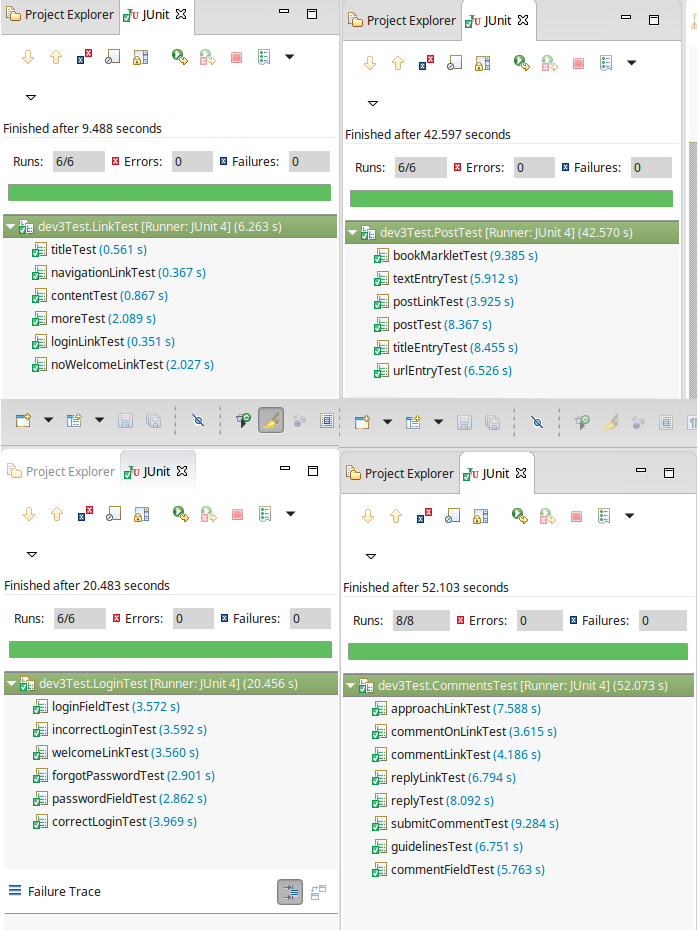
\includegraphics[width=\textwidth,natwidth=698,natheight=930]{AllTests.png}
\end{document}